\chapter{\babTiga}
Setelah masa penilaian diri selesai, pengelola dapat mengunduh hasilnya untuk dilakukan pengolahan lebih lanjut. Untuk dapat melakukannya, pengelola dapat memulainya dari menu \texttt{Overview} di sisi kiri seperti terlihat di \figurename~\ref{fig:unduhHasil}. Kemudian, di sisi kanannya terdapat menu \texttt{Responses}. Pilih sub menu \texttt{Responses \& statistics} untuk memunculkan menu seperti \figurename~\ref{fig:unduhHasil1}. 

\begin{figure}
  \begin{center}
    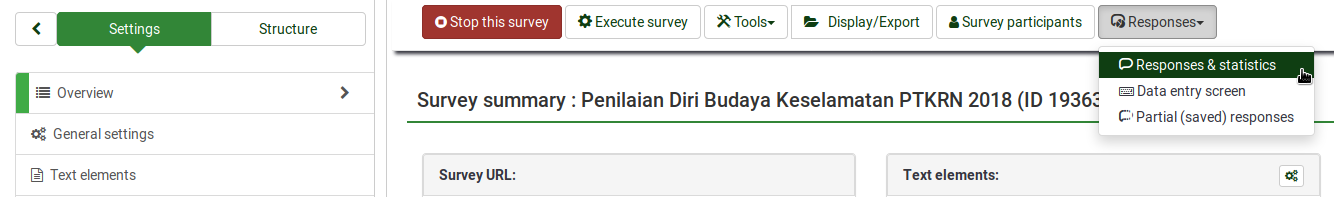
\includegraphics[scale=.25]{pics/unduhHasil.png}
    \caption{Menu yang perlu dipilih untuk menuju tahapan mengunduh hasil penilaian diri}
    \label{fig:unduhHasil}
  \end{center}
\end{figure}

\begin{figure}
  \begin{center}
    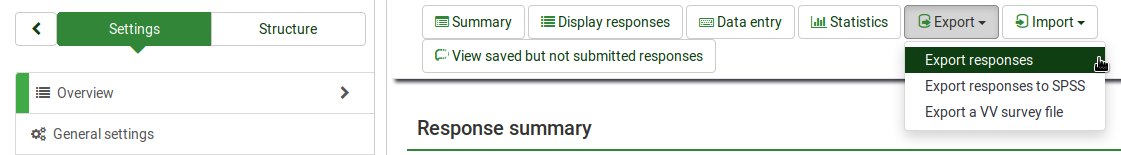
\includegraphics[scale=.35]{pics/unduhHasil1.png}
    \caption{Menu untuk mengunduh hasil penilaian diri}
    \label{fig:unduhHasil1}
  \end{center}
\end{figure}

Selanjutnya, pengelola dapat melakukan klik menu \texttt{Export responses} dan dialog seperti \figurename~\ref{fig:unduhHasil2} akan muncul.

\begin{figure}
  \begin{center}
    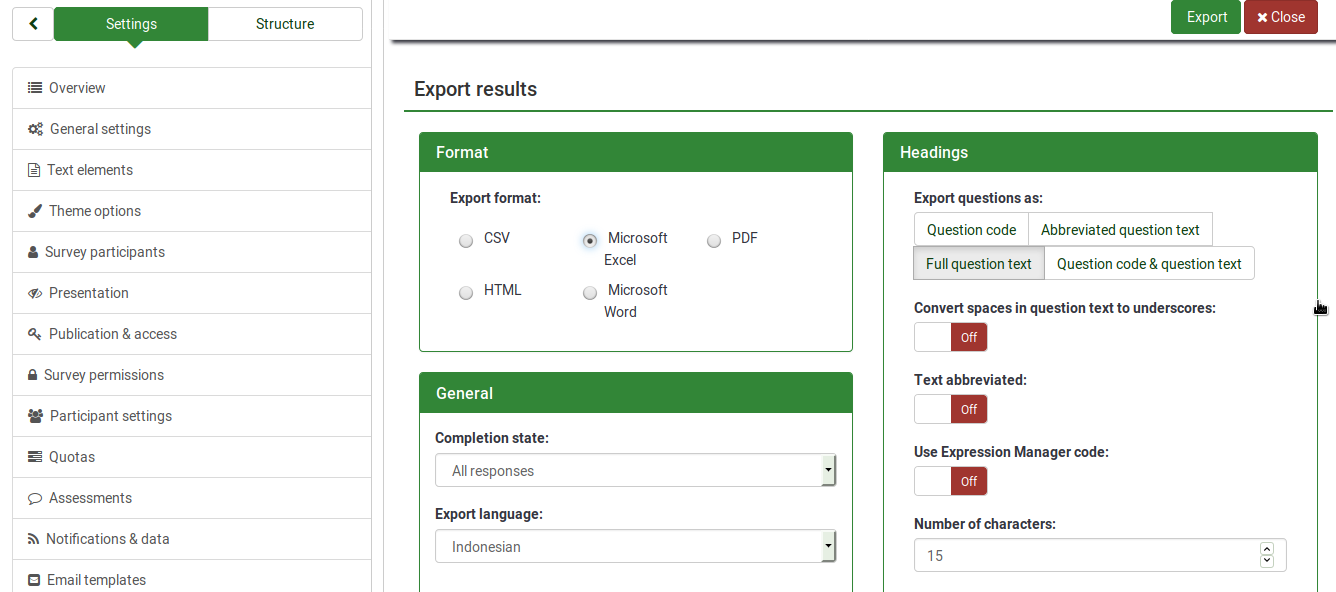
\includegraphics[scale=.25]{pics/dialogUnduhan.png}
    \caption{Dialog untuk mengunduh hasil penilaian diri dalam bentuk yang diinginkan}
    \label{fig:unduhHasil2}
  \end{center}
\end{figure}

Beberapa konfigurasi yang mungkin diperlukan adalah sebagai berikut.
\begin{enumerate}
  \item Format Microsoft Excel \textregistered~seperti \figurename~\ref{fig:excel}.\\
  \begin{figure}
    \begin{center}
      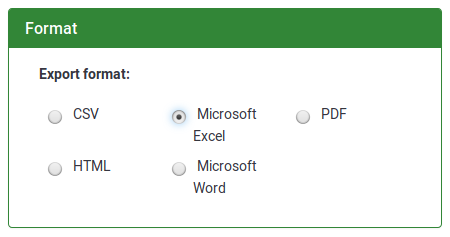
\includegraphics[scale=.5]{pics/formatExcel.png}
      \caption{Mengunduh hasil penilaian diri dengan format Microsoft Excel\textregistered}
      \label{fig:excel}
    \end{center}
  \end{figure}
  \item Hasil penilaian diri diunduh dengan format kode jawaban, buka jawaban panjang seperti \texttt{Setuju} atau \texttt{Sangat Setuju} (\figurename~\ref{fig:kodeJawaban}).\\
  \begin{figure}
    \begin{center}
      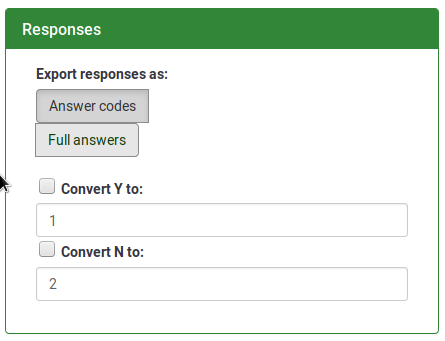
\includegraphics[scale=.5]{pics/kodeJawaban.png}
      \caption{Mengunduh hasil penilaian diri dalam bentuk kode jawaban}
      \label{fig:kodeJawaban}
    \end{center}
  \end{figure}
  \item Kolom hasil apa saja yang ingin diunduh (\figurename~\ref{fig:kolomHasil}).\\
  \begin{figure}
    \begin{center}
      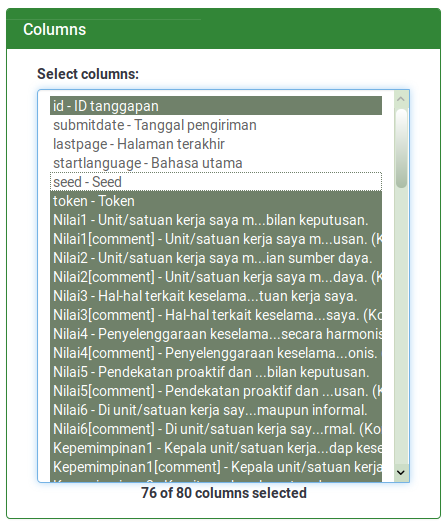
\includegraphics[scale=.5]{pics/kolomHasil.png}
      \caption{Kolom hasil yang ingin diunduh}
      \label{fig:kolomHasil}
    \end{center}
  \end{figure}
  \item Format pertanyaan yang akan menjadi label setiap kolom saat hasil penilaian diri diunduh (\figurename~\ref{fig:formatPertanyaan}).\\
  \begin{figure}
    \begin{center}
      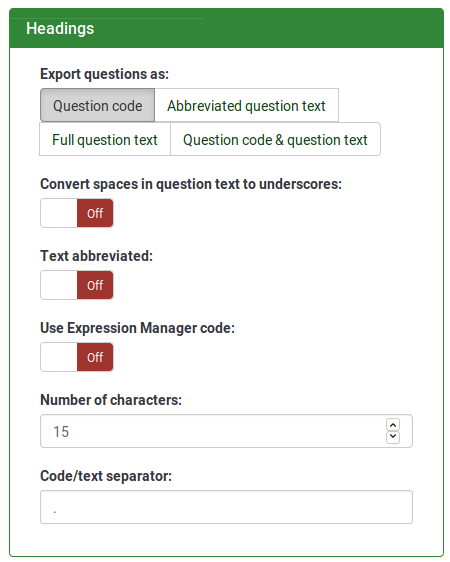
\includegraphics[scale=.5]{pics/formatPertanyaan.png}
      \caption{Format pertanyaan sebagai label kolom hasil penilaian diri}
      \label{fig:formatPertanyaan}
    \end{center}
  \end{figure}
\end{enumerate}
